% ===========================================================================
\section{Introduction}\label{sec:intro}
% ===========================================================================
Merchant ships, fishing fleets and offshore platforms now carry dense Internet of Things (IoT) installations that monitor engines, cargo, emissions, hull stress and the surrounding ocean\cite{xia2020,alqurashi2023,shang2025}. Much of this traffic is time critical. An engine alarm, a reefer-container temperature excursion or a man-overboard beacon is useful only if it reaches shore within seconds, yet ships spend most of their time beyond the reach of terrestrial networks\cite{chen2021ch,nomikos2024}. Low Earth orbit (LEO) mega-constellations are changing this picture: they offer broadband rates and tens of milliseconds of latency on the open sea\cite{kodheli2021,michel2022,laniewski2024}, and the third-generation partnership project (3GPP) has integrated non-terrestrial networks into fifth-generation standards\cite{lin2021}. Integrated space, air, ground and sea architectures are therefore a central element of sixth-generation network design\cite{liu2018,guo2022,hu2026}.

A vessel link to a LEO satellite is, however, far less predictable than a terrestrial one. The satellite moves across the sky in minutes and must be handed over before it sets\cite{wu2019,chen2024ho,chen2026sr}; Doppler and channel conditions change continuously\cite{pan2020,zhu2022}; rain cells attenuate Ku- and Ka-band signals; superstructure masts and funnels block parts of the sky; and the ship rolls and pitches with the sea, so a deck-mounted phased array scans away from its optimum and suffers motion-induced pointing loss\cite{weerackody2006}. Very-high-frequency data exchange and coastal cellular links help only near shore\cite{gomez2018}. The gateway on board must nevertheless decide, every few tens of seconds, which link to use and how aggressively to transmit.

Machine learning can predict link quality from geometry, motion and history, and recent work applies learning to handover and resource management\cite{chen2024ho,chen2026sr}. Yet every predictor is sometimes wrong, and a wrong aggressive decision means a lost critical message. What an operator needs is not a better average prediction but a guarantee: the gateway should act on a prediction only when it is safe to do so, and otherwise fall back to a robust mode, with a provable bound on how often an accepted decision fails. Selective prediction, also called learning with a reject option, provides this abstention mechanism\cite{chow1970,hendrickx2024}, and distribution-free calibration provides finite-sample guarantees\cite{vovk2022,angelopoulos2023,bates2021,angelopoulos2025}. Conformal methods have recently been applied to wireless problems\cite{cohen2023}, but no work combines them with physics-aware link prediction for maritime satellite IoT.

This paper introduces SeaSel, a certified selective link-prediction framework for maritime IoT over LEO satellite networks. Its contributions are as follows.
\begin{enumerate}
\item A formulation of maritime link selection as risk-constrained selective prediction, in which the deadline-miss rate of critical IoT messages is bounded through a certified selective risk (Section~\ref{sec:problem}).
\item A physics-biased attention ensemble that reasons jointly over all visible satellites and coastal links, with an attention bias derived from the angular separation of links, so that links sharing rain cells, blockage sectors and motion-induced scan loss exchange evidence. It is the best-calibrated predictor tested and transfers evidence across links when per-link history is missing (Section~\ref{sec:arch}).
\item A certification procedure based on Learn-then-Test with exact binomial p-values that selects the abstention threshold and the uncertainty penalty with a finite-sample guarantee, together with sea-state-conditional and online variants for distribution shift (Sections~\ref{sec:algo} and \ref{sec:uq}).
\item An open sandbox testbed that simulates a two-shell constellation, vessel routes, sea-state-driven ship motion, rain, blockage, fading and handover, used for an extensive evaluation including ablation, robustness and out-of-distribution analyses (Sections~\ref{sec:setup}--\ref{sec:ablation}).
\end{enumerate}
Unlike work that tunes a better predictor or a better handover rule, SeaSel changes the decision interface between learning and radio control: the radio acts only on certified predictions, and the certificate carries an explicit reliability guarantee for the IoT service.

% ===========================================================================
\section{Related work}\label{sec:related}
% ===========================================================================
\subsection{Maritime IoT and satellite--terrestrial connectivity}
Surveys of maritime communication describe a heterogeneous mix of shore-based cellular systems, very-high-frequency data exchange, geostationary and non-geostationary satellites, and aerial relays\cite{alqurashi2023,shang2025,xia2020}. Xia \emph{et al.}\cite{xia2020} identify intermittent coverage, limited spectrum and the harsh marine environment as the main obstacles to a maritime IoT, and Alqurashi \emph{et al.}\cite{alqurashi2023} survey enabling technologies from visible-light to satellite links. Channel measurement studies show that sea-surface reflection, evaporation ducts and platform motion make maritime channels distinct from terrestrial ones\cite{chen2021ch}. Integrated architectures that combine space, air and ground segments have been proposed for global coverage\cite{liu2018,guo2022}, and recent studies analyse LEO and unmanned-aerial-vehicle assistance for maritime data collection\cite{hu2026,nomikos2024}. Field trials of the satellite component of the very-high-frequency data exchange system demonstrate low-rate maritime satellite messaging\cite{gomez2018}. These works establish the connectivity options available to a vessel but treat link selection with static rules or average performance models.

\subsection{LEO link dynamics, measurement and handover}
The new space era has produced constellations of thousands of LEO satellites\cite{kodheli2021}, and 3GPP release 17 standardised non-terrestrial access for fifth-generation systems\cite{lin2021}. Measurement campaigns show that Starlink throughput and latency vary strongly with time, obstruction and motion; Michel \emph{et al.}\cite{michel2022} report a first look at stationary performance, and Laniewski \emph{et al.}\cite{laniewski2024} show that mobile terminals experience frequent outages caused by obstructions and handovers. Channel characterisation for Ka-band LEO IoT\cite{zhu2022} and Doppler estimation and compensation\cite{pan2020} address physical-layer impairments. Motion-induced antenna pointing error is a known problem for satellite communication on the move\cite{weerackody2006}. Handover strategies based on potential games\cite{wu2019}, soft actor-critic learning\cite{chen2024ho} and graph-guided multi-agent deep Q-networks\cite{chen2026sr} choose the next serving satellite to maximise throughput or minimise handover frequency. These methods optimise expected performance; none of them provides a guarantee on the failure probability of the decisions it takes.

\subsection{Learning-based prediction and attention}
Deep learning is widely used for link-quality and handover prediction, and attention mechanisms have become the standard tool for relating elements of a set or sequence\cite{brauwers2023}. For a vessel gateway, the natural input is a variable-size set of candidate links whose outcomes are correlated: links pointing to nearby parts of the sky share rain cells, blockage sectors and scan loss. Generic attention ignores this physical structure and must learn it from data, while per-link classifiers ignore it entirely. Uncertainty quantification for deep learning has been reviewed extensively\cite{abdar2021}; deep ensembles and temperature scaling are among the most reliable practical techniques, but on their own they provide no finite-sample guarantee. Learned handover controllers\cite{chen2024ho,chen2026sr} use reward-driven policies whose occasional failures are averaged into the return rather than bounded, and measurement studies of mobile LEO terminals\cite{laniewski2024} show that such failures cluster in time, exactly when a vessel enters a storm or turns its superstructure towards the serving satellite. A predictor for this setting therefore needs three properties at once: it must handle a variable set of candidates, exploit their correlation, and expose a calibrated confidence that a downstream controller can threshold.

\subsection{Selective prediction and distribution-free risk control}
Chow's reject option\cite{chow1970} established the trade-off between error and rejection, and Hendrickx \emph{et al.}\cite{hendrickx2024} survey modern learning with a reject option. Conformal prediction provides distribution-free coverage guarantees under exchangeability\cite{vovk2022,angelopoulos2023}. Risk-controlling prediction sets\cite{bates2021} and the Learn-then-Test framework\cite{angelopoulos2025} extend these guarantees to general risks through multiple hypothesis testing, and conformal prediction beyond exchangeability addresses distribution drift\cite{barber2023}. Concentration inequalities such as Hoeffding's\cite{hoeffding1963} underlie many of these bounds. In wireless communications, Cohen \emph{et al.}\cite{cohen2023} calibrate demodulation and modulation-classification models with conformal prediction. Exchangeability, the key assumption of these guarantees, is fragile in the ocean: sea state, rain regime and constellation health change over hours to months, and Barber \emph{et al.}\cite{barber2023} show that coverage degrades gracefully only in proportion to the size of the shift. Practical systems therefore need both a certificate and a mechanism that detects and corrects drift. These methods have not been applied to link selection for maritime satellite IoT, where the abstention action has a physical meaning (switching to a robust transmission mode) and the risk to be controlled is the failure rate of accepted transmissions.

\subsection{Problem statements and research gaps}
The review leads to four problem statements.
\textbf{PS1.} A vessel gateway must choose among a changing set of satellite and coastal links whose success depends jointly on orbital geometry, ship motion, weather and superstructure blockage.
\textbf{PS2.} Critical IoT messages require a bounded failure probability, but learned link predictors are fallible and their errors are not controlled.
\textbf{PS3.} Link outcomes are correlated across candidates in a way determined by geometry, which per-link models cannot exploit.
\textbf{PS4.} Sea state, weather regime and constellation health drift over time, so a guarantee calibrated on past data may silently fail.

The corresponding research gaps are:
\textbf{RG1.} No existing maritime or LEO handover method provides a finite-sample guarantee on the failure rate of the link decisions it accepts\cite{wu2019,chen2024ho,chen2026sr}.
\textbf{RG2.} Selective prediction and risk control\cite{bates2021,angelopoulos2025,hendrickx2024} have not been connected to a physical fallback mode in satellite IoT, so the operational meaning of abstention is undefined.
\textbf{RG3.} Attention models for link prediction do not encode the geometric coupling between links\cite{brauwers2023}.
\textbf{RG4.} The robustness of certified link decisions to maritime distribution shift (storms, tropical rain, satellite failures) has not been studied.
SeaSel addresses RG1 and RG2 through certified selective prediction with a dual-link robust fallback, RG3 through physics-biased attention, and RG4 through sea-state-conditional and online risk control, evaluated on a reproducible testbed.

% ===========================================================================
\section{Problem formulation and motivation for selective prediction}\label{sec:problem}
% ===========================================================================
\subsection{System model}
Figures~\ref{fig:physical}--\ref{fig:temporal} show the system from three viewpoints. The physical view (Fig.~\ref{fig:physical}) contains a set $\mathcal V$ of vessels, each carrying IoT sensors and a gateway with a deck-mounted phased array and, near ports, a fifth-generation modem. Two Walker constellation shells provide coverage; a moving rain cell, the ship's roll and the masts determine which links are usable. The functional view (Fig.~\ref{fig:functional}) shows the layered gateway software, and the temporal view (Fig.~\ref{fig:temporal}) shows how training, calibration and deployment are arranged in time. Table~\ref{tab:symbols} lists the notation.

\begin{figure}[t]
\centering
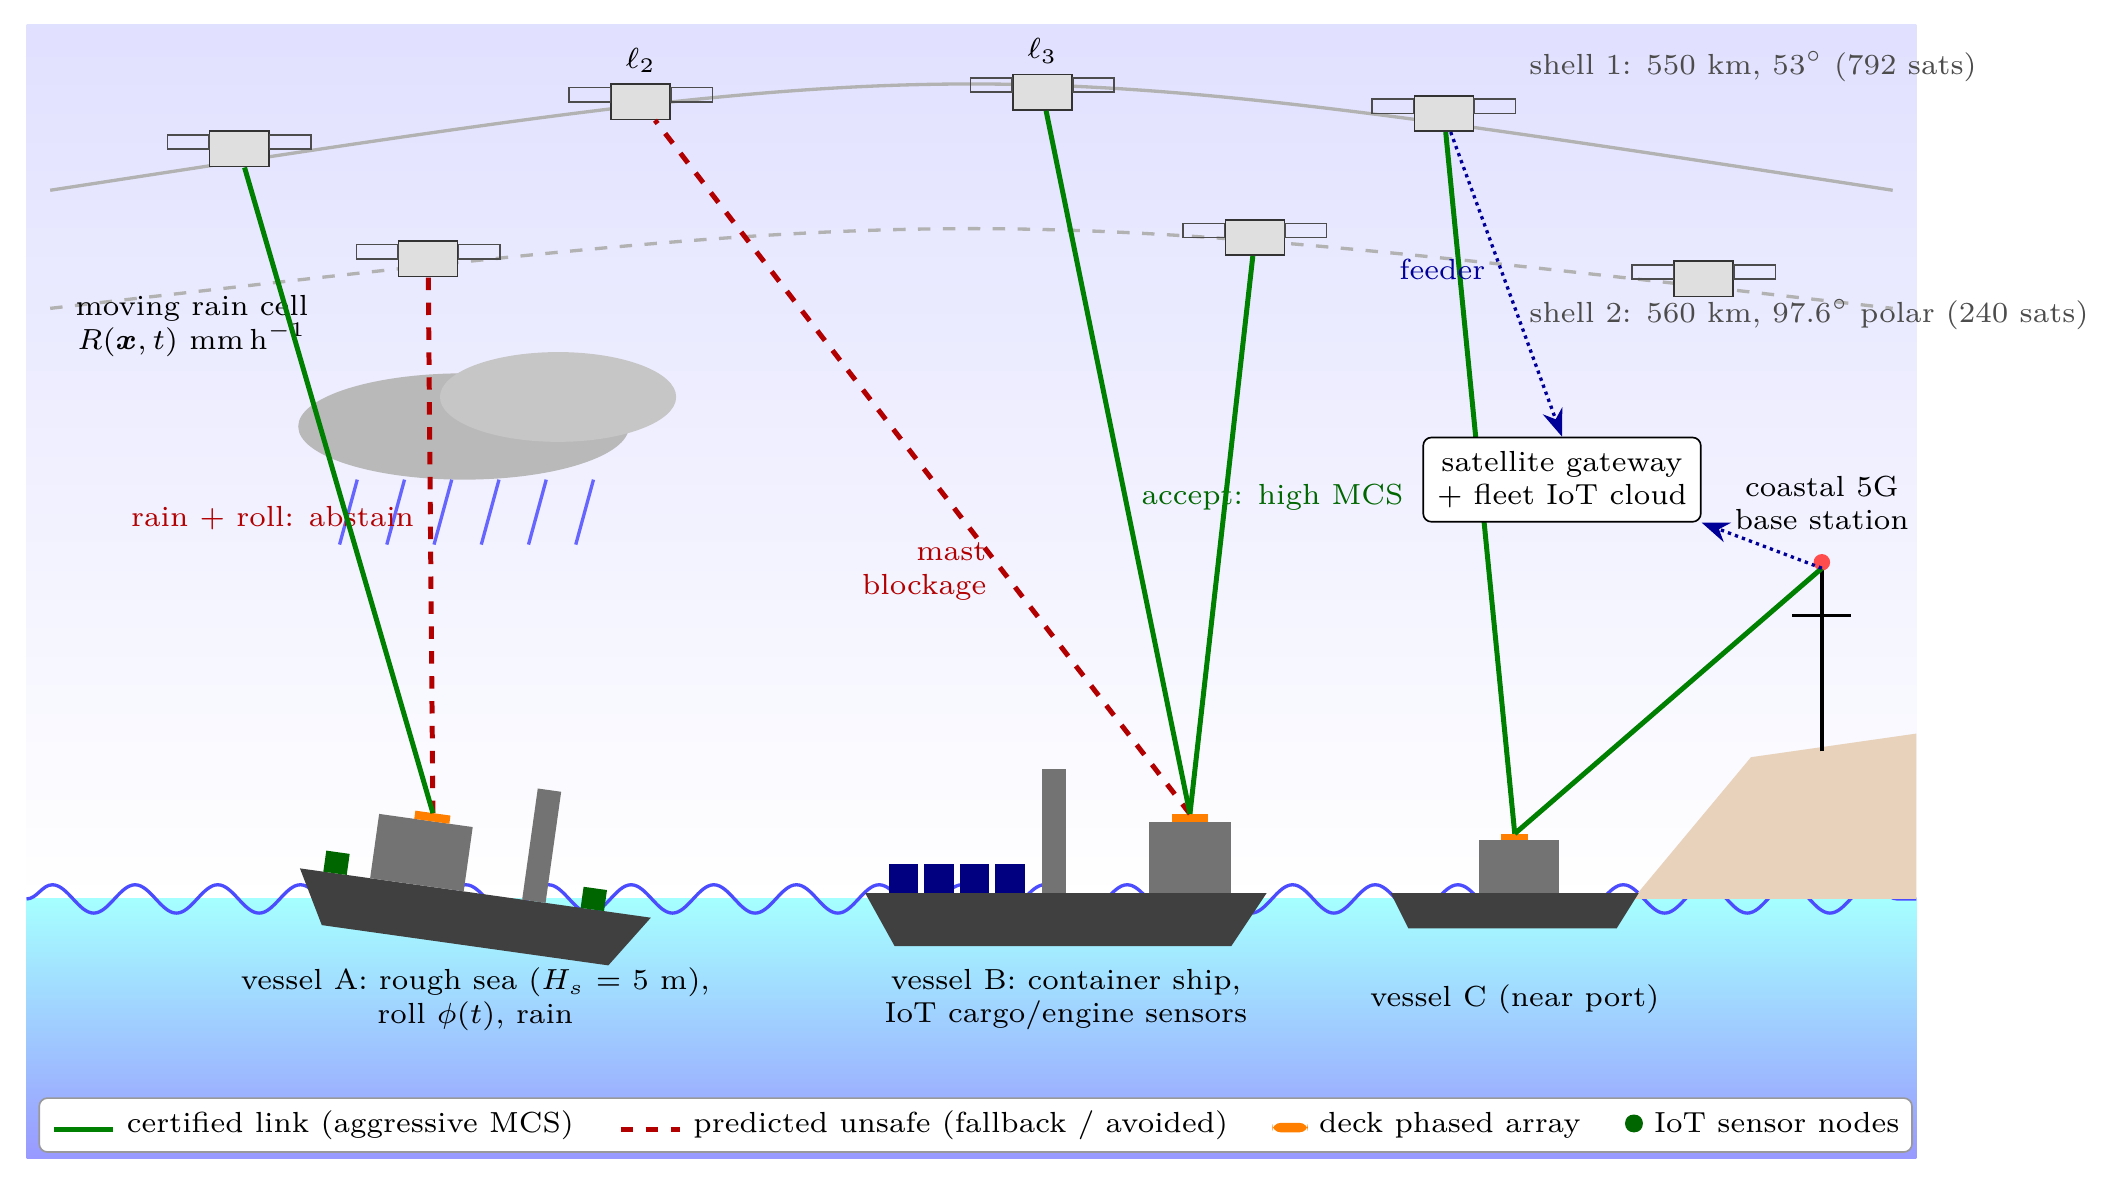
\includegraphics[width=\textwidth]{../figures/diagrams/sys_physical.png}
\caption{\textbf{Physical view of the maritime IoT satellite system.} Vessels select among visible LEO satellites of two shells and a coastal fifth-generation base station. Rain cells, ship roll and mast blockage make some links unsafe; certified links are used with an aggressive modulation and coding scheme, and unsafe decisions trigger the robust fallback.}
\label{fig:physical}
\end{figure}

\begin{figure}[t]
\centering
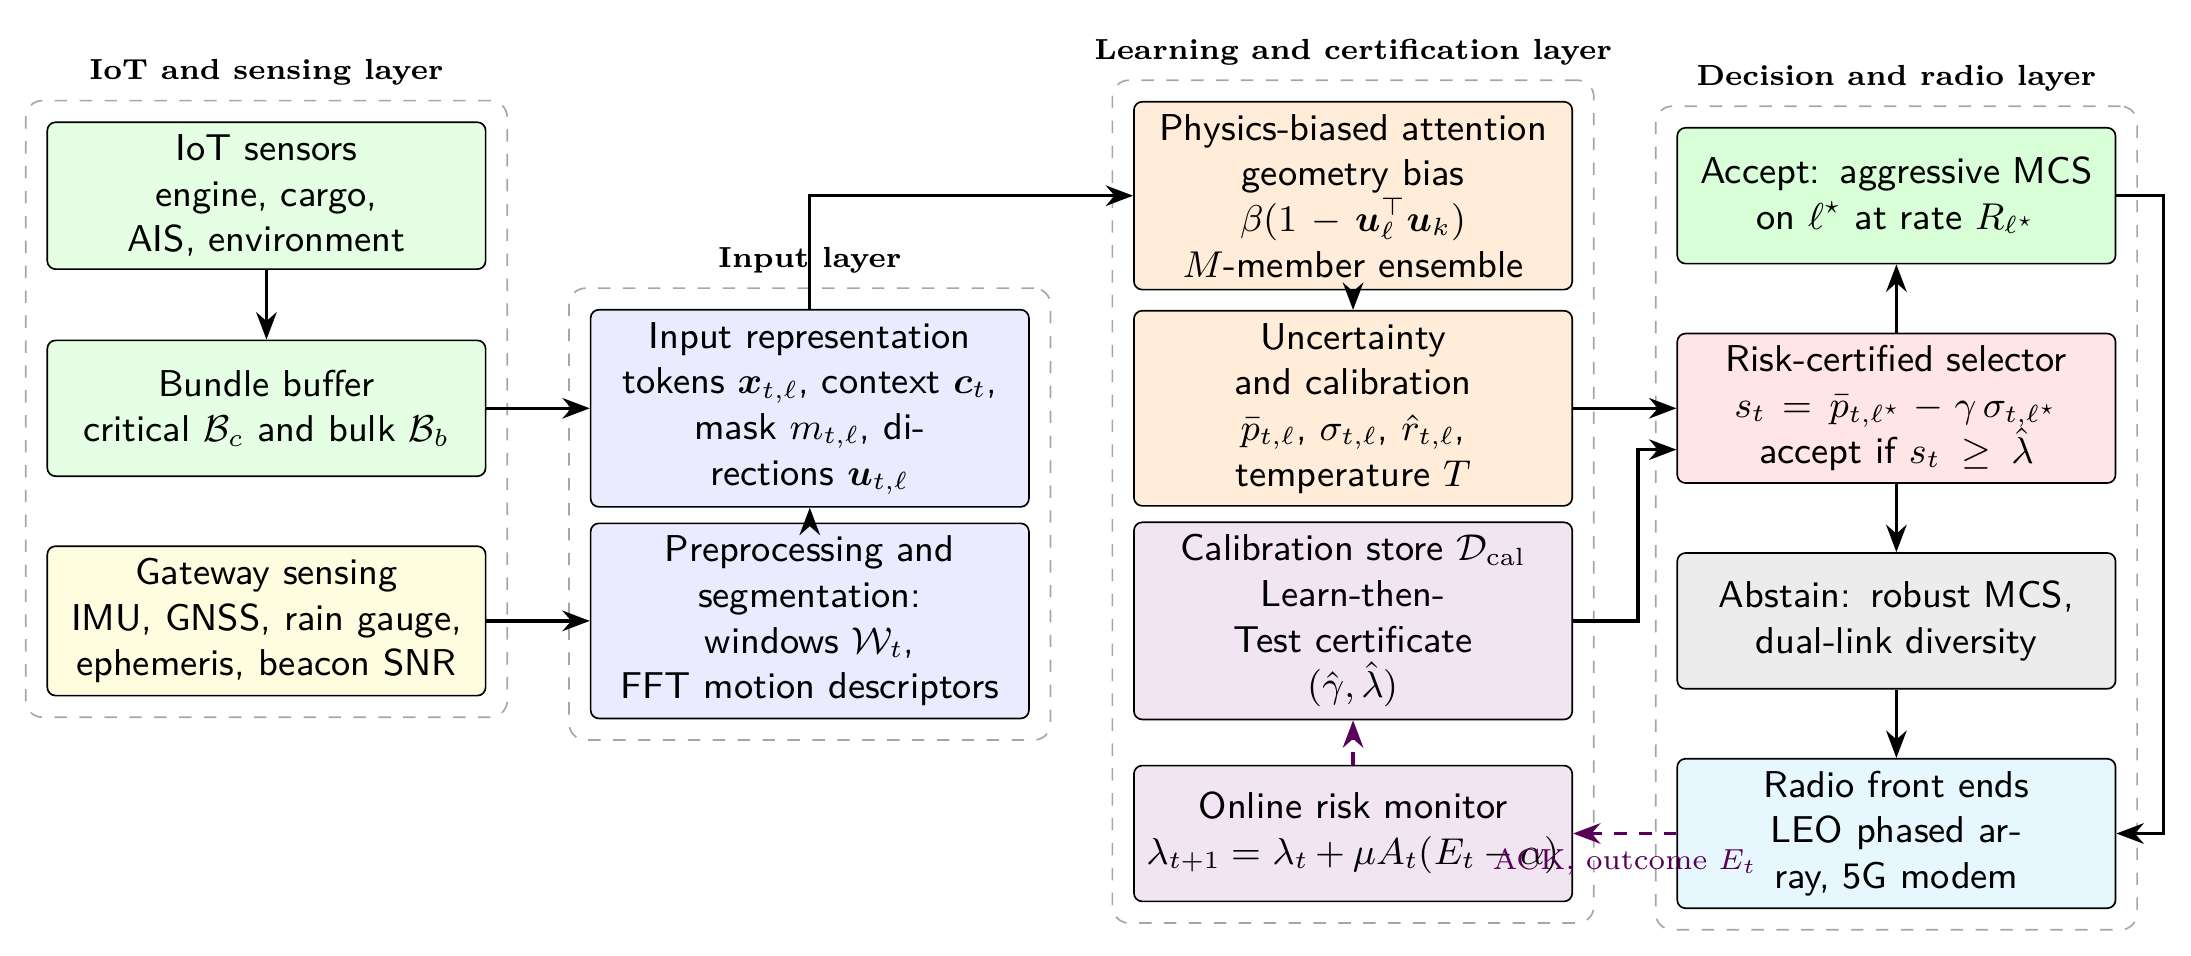
\includegraphics[width=\textwidth]{../figures/diagrams/sys_functional.png}
\caption{\textbf{Functional view of the SeaSel gateway.} Sensing data are segmented and tokenised, a physics-biased attention ensemble estimates link-success probabilities and their uncertainty, and a risk-certified selector either accepts an aggressive transmission or abstains to a robust dual-link mode. Outcomes feed the calibration store and the online risk monitor.}
\label{fig:functional}
\end{figure}

\begin{figure}[t]
\centering
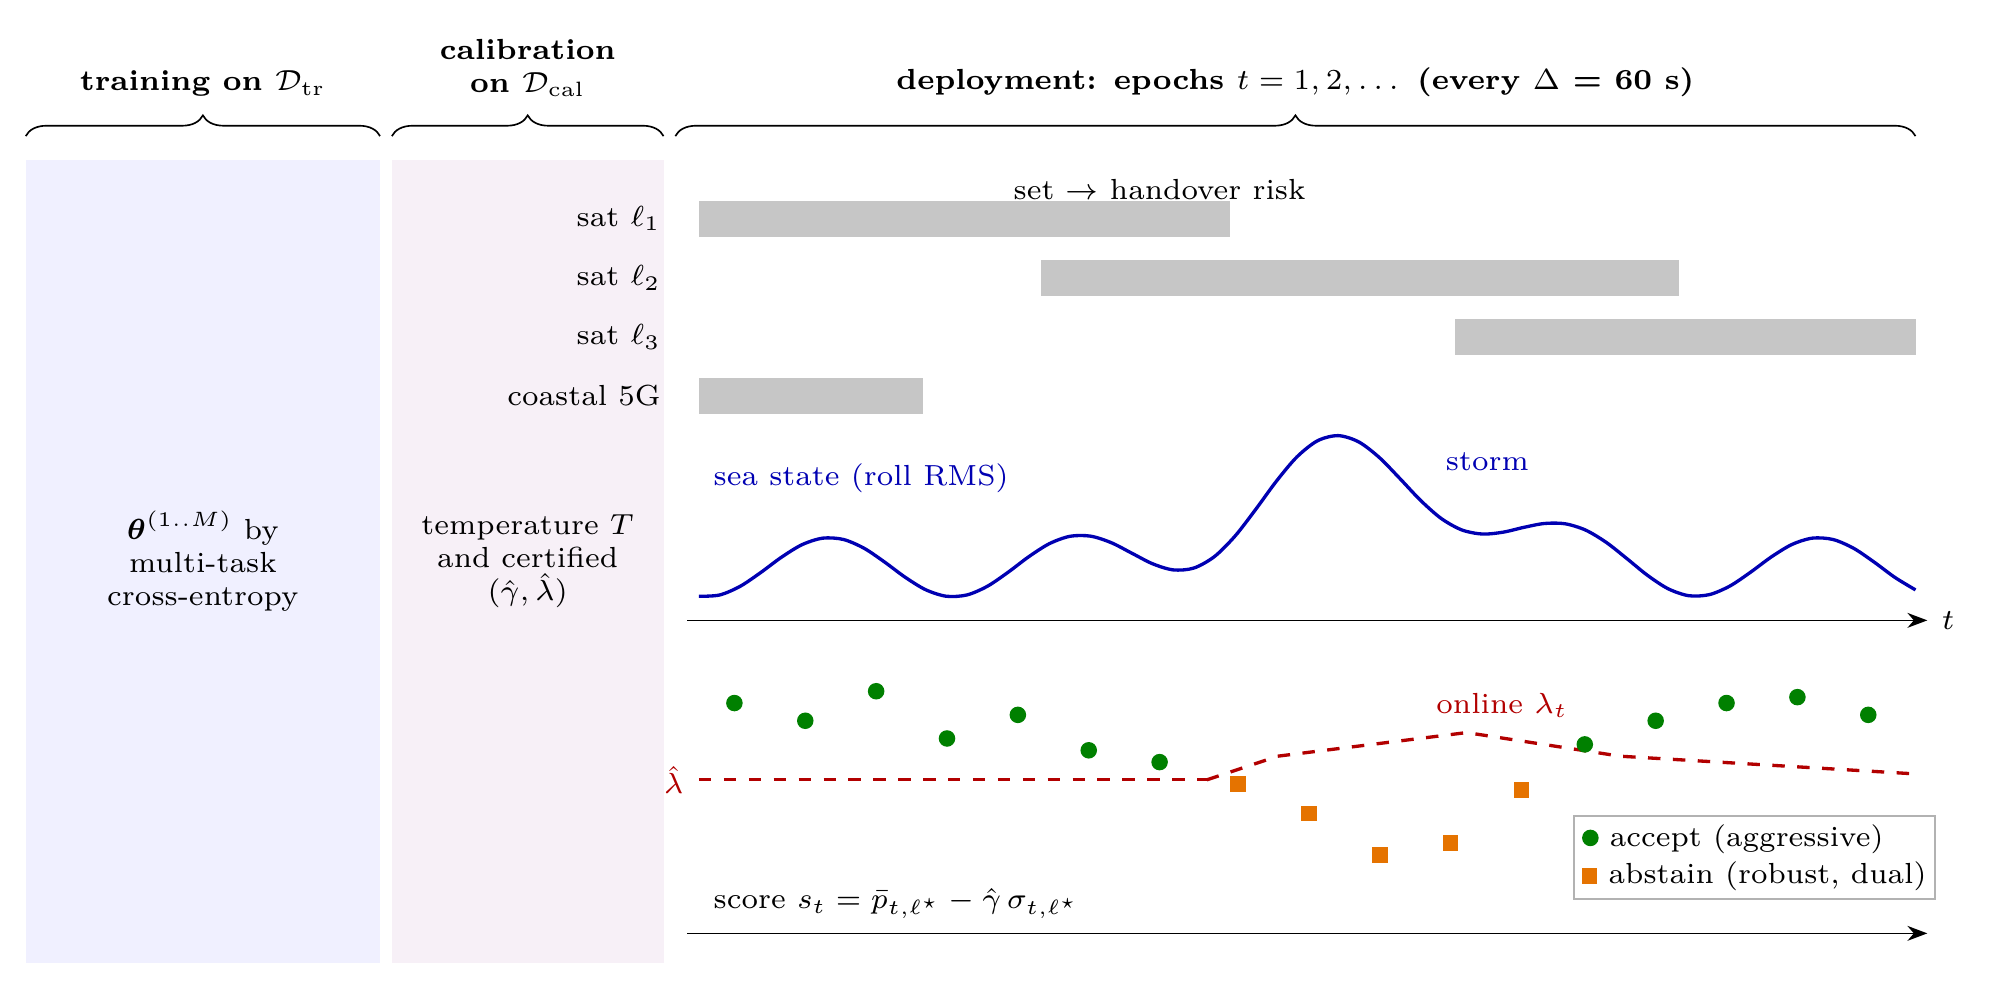
\includegraphics[width=\textwidth]{../figures/diagrams/sys_temporal.png}
\caption{\textbf{Temporal view of training, calibration and deployment.} During deployment the certified score $s_t$ is compared with the threshold $\hat\lambda$; when a storm degrades link quality, scores fall below the threshold and the gateway abstains, while the online monitor raises $\lambda_t$ if accepted decisions start to fail.}
\label{fig:temporal}
\end{figure}

Time is divided into decision epochs of duration $\Delta$. At epoch $t$, the gateway of vessel $v$ sees a candidate set $\mathcal L_t$ of at most $K$ satellites above the minimum elevation $\theta_{\min}$ plus, when within range, one coastal link. For a satellite link $\ell$ at range $d_{t,\ell}$ and elevation $\theta_{t,\ell}$, the signal-to-noise ratio of a transmission of duration $T_x$ is modelled as
\begin{equation}\label{eq:snr}
\mathrm{SNR}_{t,\ell}=\mathrm{SNR}_{\rm ref}-20\log_{10}\frac{d_{t,\ell}}{h_{\rm s}}-L^{\rm atm}_{t,\ell}-L^{\rm scan}_{t,\ell}-L^{\rm pt}_{t,\ell}-L^{\rm rain}_{t,\ell}-L^{\rm blk}_{t,\ell}+10\log_{10}|g_{t,\ell}|^{2}+\xi_{t,\ell},
\end{equation}
where $h_{\rm s}$ is the shell altitude, $g_{t,\ell}$ a Rician fading coefficient whose $K$-factor grows with elevation and $\xi_{t,\ell}$ scintillation. The deck normal $\bm n(\phi,\vartheta)$ rotates with roll $\phi$ and pitch $\vartheta$, so the scan angle of the array and the resulting scan loss are
\begin{equation}\label{eq:scan}
\cos\chi_{t,\ell}(\tau)=\bm n\big(\phi(\tau),\vartheta(\tau)\big)^{\top}\bm u^{\rm b}_{t,\ell},\qquad
L^{\rm scan}_{t,\ell}=-\frac{10\,n_{\rm s}}{T_x}\int_{t\Delta}^{t\Delta+T_x}\log_{10}\cos\chi_{t,\ell}(\tau)\,d\tau,
\end{equation}
with $\bm u^{\rm b}_{t,\ell}$ the satellite direction in the ship body frame and $n_{\rm s}$ the scan exponent. Motion also causes a tracking lag proportional to the angular rate $\omega_t$, giving the pointing loss
\begin{equation}\label{eq:pointing}
L^{\rm pt}_{t,\ell}=12\left(\frac{\kappa\,\omega_t}{\theta_{3\mathrm{dB}}}\right)^{2},
\end{equation}
where $\kappa$ is the tracking latency and $\theta_{3\mathrm{dB}}$ the beamwidth. Rain of rate $R_t$ attenuates the slant path through the rain layer of height $h_R$:
\begin{equation}\label{eq:rain}
L^{\rm rain}_{t,\ell}=a R_t^{\,b}\,\frac{L_s}{1+L_s\cos\theta_{t,\ell}/L_0},\qquad L_s=\frac{h_R}{\sin\theta_{t,\ell}}.
\end{equation}
A transmission succeeds in the aggressive mode, with rate $R_\ell$, or in the robust mode, with rate $R_0\ll R_\ell$, when
\begin{equation}\label{eq:labels}
Y_{t,\ell}=\mathbb 1\{\mathrm{SNR}_{t,\ell}\ge\eta_A\}\,\mathbb 1\{\theta_{t,\ell}(t\Delta+T_x)\ge\theta_{\min}\},\qquad
Y^{R}_{t,\ell}=\mathbb 1\{\mathrm{SNR}_{t,\ell}\ge\eta_R\}\,\mathbb 1\{\theta_{t,\ell}(t\Delta+T_x)\ge\theta_{\min}\},
\end{equation}
where the second factor captures handover failure when the satellite sets during the transmission.

\subsection{Traffic, transmission and feedback model}
Each vessel generates two traffic classes. A critical bundle $\mathcal B_c$ of a few kilobytes (alarms, safety telemetry, compliance reports) must be delivered within the epoch in which it is created; a bulk bundle $\mathcal B_b$ (engine logs, cargo telemetry, environmental sensor streams) is delay tolerant and benefits from every additional megabit. In each epoch the gateway makes a single transmission decision of duration $T_x$. In the aggressive mode it sends both bundles over one link with a high-order modulation and coding scheme; in the robust mode it sends the critical bundle, and as much bulk data as the low rate allows, over the two most reliable links with a low-order scheme, which doubles the radiated energy. Satellites and the coastal base station acknowledge every transmission, so the outcome $E_t$ of an accepted decision is known at the end of the epoch. This feedback is what makes the online rule of Section~\ref{sec:uq} possible. The gateway knows the ephemeris of every satellite, its own position and heading, its inertial measurements and the beacon SNR of the satellites it tracked in the previous epoch; it does not know the instantaneous rain field, the fading state or the exact roll during the transmission. Two assumptions underpin the guarantees: calibration and deployment epochs are exchangeable unless stated otherwise, and acknowledgements are reliable, which is reasonable because they are short and can be sent with the most robust scheme.

\subsection{Selective decision model}
Let $\bar p_{t,\ell}$ be the predicted aggressive-success probability, $\sigma_{t,\ell}$ its epistemic uncertainty and $\hat r_{t,\ell}$ the predicted robust-success probability. The gateway chooses the link with the highest expected aggressive goodput and forms an uncertainty-penalised confidence score:
\begin{equation}\label{eq:choice}
\ell^\star_t=\arg\max_{\ell\in\mathcal L_t}\ \bar p_{t,\ell}R_\ell,\qquad
s_t(\gamma)=\bar p_{t,\ell^\star_t}-\gamma\,\sigma_{t,\ell^\star_t},
\end{equation}
and accepts the aggressive transmission only when the score clears a threshold:
\begin{equation}\label{eq:accept}
A_t(\gamma,\lambda)=\mathbb 1\{s_t(\gamma)\ge\lambda\}.
\end{equation}
When $A_t=0$ the gateway abstains and sends the critical bundle in the robust mode duplicated over the two links with the highest $\hat r_{t,\ell}$, which costs twice the energy. Writing $E_t=1-Y_{t,\ell^\star_t}$ for an aggressive failure and $F_t$ for a failure of the robust fallback, the selective risk, the critical-message miss rate and the goodput are
\begin{equation}\label{eq:selrisk}
R_{\rm sel}(\gamma,\lambda)=\Pr\big[E_t=1\mid A_t(\gamma,\lambda)=1\big],
\end{equation}
\begin{equation}\label{eq:miss}
\mathcal M(\gamma,\lambda)=\Pr[A_t=1,E_t=1]+\Pr[A_t=0,F_t=1],
\end{equation}
\begin{equation}\label{eq:goodput}
\mathcal G(\gamma,\lambda)=T_x\,\mathbb E\big[A_t(1-E_t)R_{\ell^\star_t}+(1-A_t)(1-F_t)R_0\big].
\end{equation}

\subsection{Risk-constrained objective}
The design problem is to maximise goodput while guaranteeing that accepted aggressive transmissions fail rarely:
\begin{equation}\label{eq:objective}
\max_{\gamma,\lambda}\ \mathcal G(\gamma,\lambda)\quad\text{subject to}\quad \Pr_{\mathcal D_{\rm cal}}\big[R_{\rm sel}(\hat\gamma,\hat\lambda)\le\alpha\big]\ge1-\delta,
\end{equation}
where the probability is over the random calibration set $\mathcal D_{\rm cal}$, $\alpha$ is the tolerated selective risk and $\delta$ the confidence parameter. Because the coverage $c=\Pr[A_t=1]$ and the fallback failure probability $\rho_F=\Pr[F_t=1\mid A_t=0]$ are measurable, constraint (\ref{eq:objective}) bounds the miss rate directly:
\begin{equation}\label{eq:missbound}
\mathcal M\le c\,\alpha+(1-c)\,\rho_F .
\end{equation}

\subsection{Motivation for selective prediction}
Two naive designs bracket the problem. Always transmitting aggressively maximises goodput but lets every prediction error become a lost critical message. Always transmitting robustly protects critical messages but reduces goodput by an order of magnitude and doubles energy per bit. Tuning a confidence threshold on validation data sits in between, but its risk is uncontrolled: the threshold is a point estimate and can exceed the target on new data, as the experiments confirm. Selective prediction with certification resolves this tension. The predictor acts where it is reliable, abstains where it is not, and the certificate (\ref{eq:objective}) turns the abstention threshold into an engineering parameter with a guaranteed meaning. Through bound (\ref{eq:missbound}) it also converts a statistical guarantee into a service-level guarantee for maritime IoT. As an illustration, with $\alpha=0.05$, a coverage of 90\% and a fallback failure probability of 2\%, the bound gives a miss rate of at most 4.7\%, while the vessel still uses the aggressive scheme in nine epochs out of ten.

\begin{table}[t]
\centering\small
\caption{\textbf{Symbols and notation.}}
\label{tab:symbols}
\begin{tabular}{@{}ll@{\hspace{1.2em}}ll@{}}
\toprule
Symbol & Meaning & Symbol & Meaning\\\midrule
$\mathcal V$, $v$ & vessels, vessel index & $t$, $\Delta$ & decision epoch, epoch duration\\
$\mathcal L_t$, $\ell$, $K$ & candidate links, link, max.\ satellites & $T_x$ & transmission duration\\
$\theta_{t,\ell}$, $d_{t,\ell}$ & elevation, slant range & $\bm u_{t,\ell}$ & unit direction to link $\ell$\\
$\phi$, $\vartheta$, $\omega_t$ & roll, pitch, angular rate & $H_s$ & significant wave height\\
$\chi_{t,\ell}$, $n_{\rm s}$ & scan angle, scan exponent & $\kappa$, $\theta_{3\mathrm{dB}}$ & tracking latency, beamwidth\\
$R_t$, $h_R$ & rain rate, rain height & $a$, $b$ & rain attenuation coefficients\\
$\eta_A$, $\eta_R$ & aggressive / robust SNR thresholds & $R_\ell$, $R_0$ & aggressive / robust rates\\
$Y_{t,\ell}$, $Y^R_{t,\ell}$ & aggressive / robust success & $\bm x_{t,\ell}$, $\bm c_t$ & link token, vessel context\\
$m_{t,\ell}$ & validity mask & $\mathcal W_t$ & IMU segment for epoch $t$\\
$\bar p_{t,\ell}$, $\sigma_{t,\ell}$ & ensemble mean, spread & $\hat r_{t,\ell}$ & robust-success probability\\
$M$, $T$ & ensemble size, temperature & $\beta$ & physics-bias strength\\
$s_t$, $\gamma$, $\lambda$ & score, uncertainty penalty, threshold & $A_t$, $E_t$, $F_t$ & accept, aggressive / fallback failure\\
$R_{\rm sel}$, $c$ & selective risk, coverage & $\mathcal M$, $\mathcal G$ & miss rate, goodput\\
$\alpha$, $\delta$ & target risk, confidence & $\mathcal D_{\rm tr}$, $\mathcal D_{\rm cal}$ & training and calibration sets\\
$\mu$ & online step size & $g(\cdot)$ & sea-state group\\
\bottomrule
\end{tabular}
\end{table}
